\documentclass[a4paper,12pt]{article}
\usepackage{CJKutf8}
\usepackage{amsthm}
\usepackage{amsmath}
\usepackage{amssymb}
\usepackage{geometry}
\usepackage{graphicx}
\usepackage{array}
\usepackage{subfigure}
\usepackage{appendix}
\usepackage{listings}
\usepackage{xcolor}
\usepackage{tikz}
\usepackage{float}
\usepackage{tcolorbox}
\usepackage[ruled,vlined,commentsnumbered]{algorithm2e}
\usepackage{multicol}
\usepackage{pgfplots}
\pgfplotsset{compat=1.17}
\usepackage{indentfirst}
\usepackage{enumitem}
\usepackage[colorlinks,linkcolor=blue,anchorcolor=blue,citecolor=blue]{hyperref}
\hypersetup{unicode} % to display the unicode char in the bookmark correctly
\usepackage{bookmark} % should be introduced after package hyperref
\setlength{\parskip}{1ex}
\setenumerate[1]{itemsep=0pt,partopsep=0pt,parsep=\parskip,topsep=5pt}
\setitemize[1]{itemsep=0pt,partopsep=0pt,parsep=\parskip,topsep=5pt}
\setdescription{itemsep=0pt,partopsep=0pt,parsep=\parskip,topsep=5pt}
\geometry{left=1.0cm,right=1.0cm,top=2.0cm,bottom=2.0cm}
\renewcommand{\figurename}{图}
\renewcommand{\tablename}{表}

\usepackage{subfigure}
\usepackage{wasysym}

\begin{document}
\begin{CJK}{UTF8}{song}
\title{高中学生作业量}
\author{LogCreative}
\date{2017/10/3}
\maketitle
\normalsize

\paragraph{1. 作业完成总量是不稳定的。} 由图\ref{avg}可以看到,由于每周的学习任务不同,总量会有所变化。三个峰值均是考试前的一周,这个值可以高出最低时的40\%以上。
由图中还可以看到,每科的量也是随之变化的,即总体占比基本不变。

\begin{figure}[H]
    \centering
    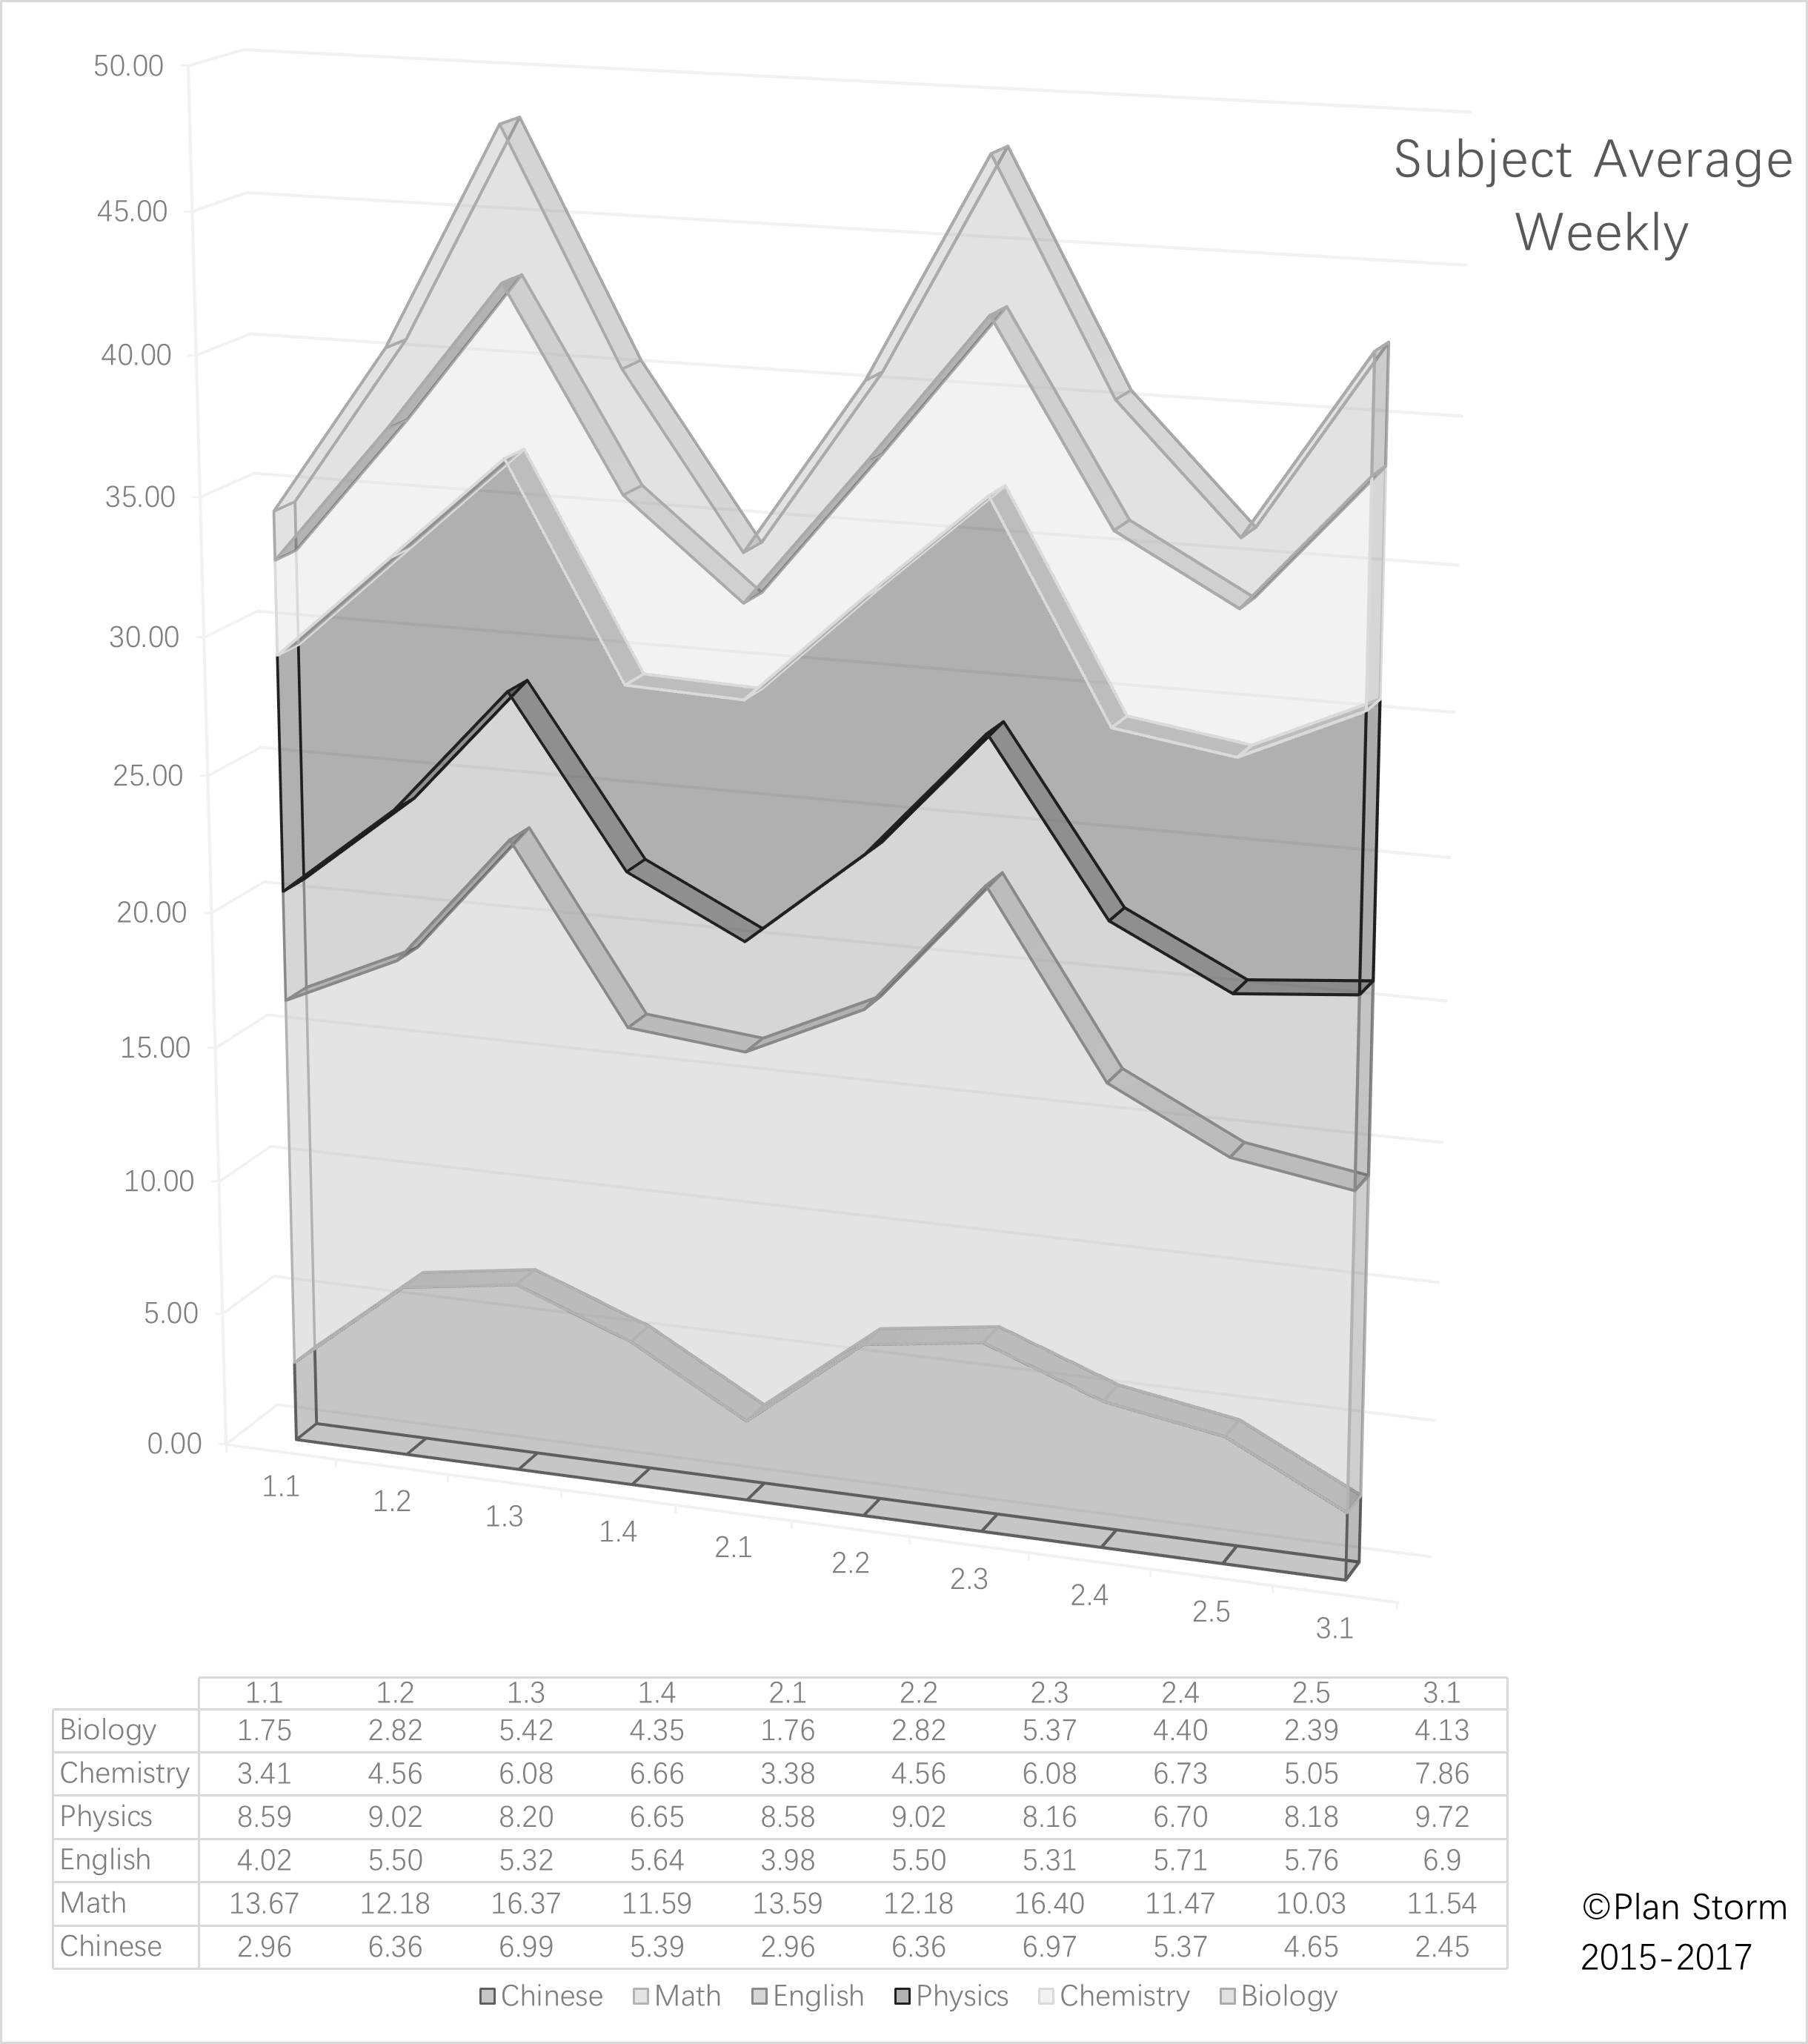
\includegraphics[height=16cm]{img/1.png}
    \caption{学科平均 Pt./week}
    \label{avg}
\end{figure}

\paragraph{2. 学科分配时间是不同的。} 根据10周的数据,可以得到如图\ref{ratio}所示的基本分布。数学和物理总占比为52\%,占据了同学大部分的时间。
同学的平均作业时间为20个小时/星期≈3-4小时/天。
由于数据量大,我们可以说,如果想要在某学科上多花点时间的话,只要比图示中的作业标准每周多一些即可。

\begin{figure}[H]
    \centering
    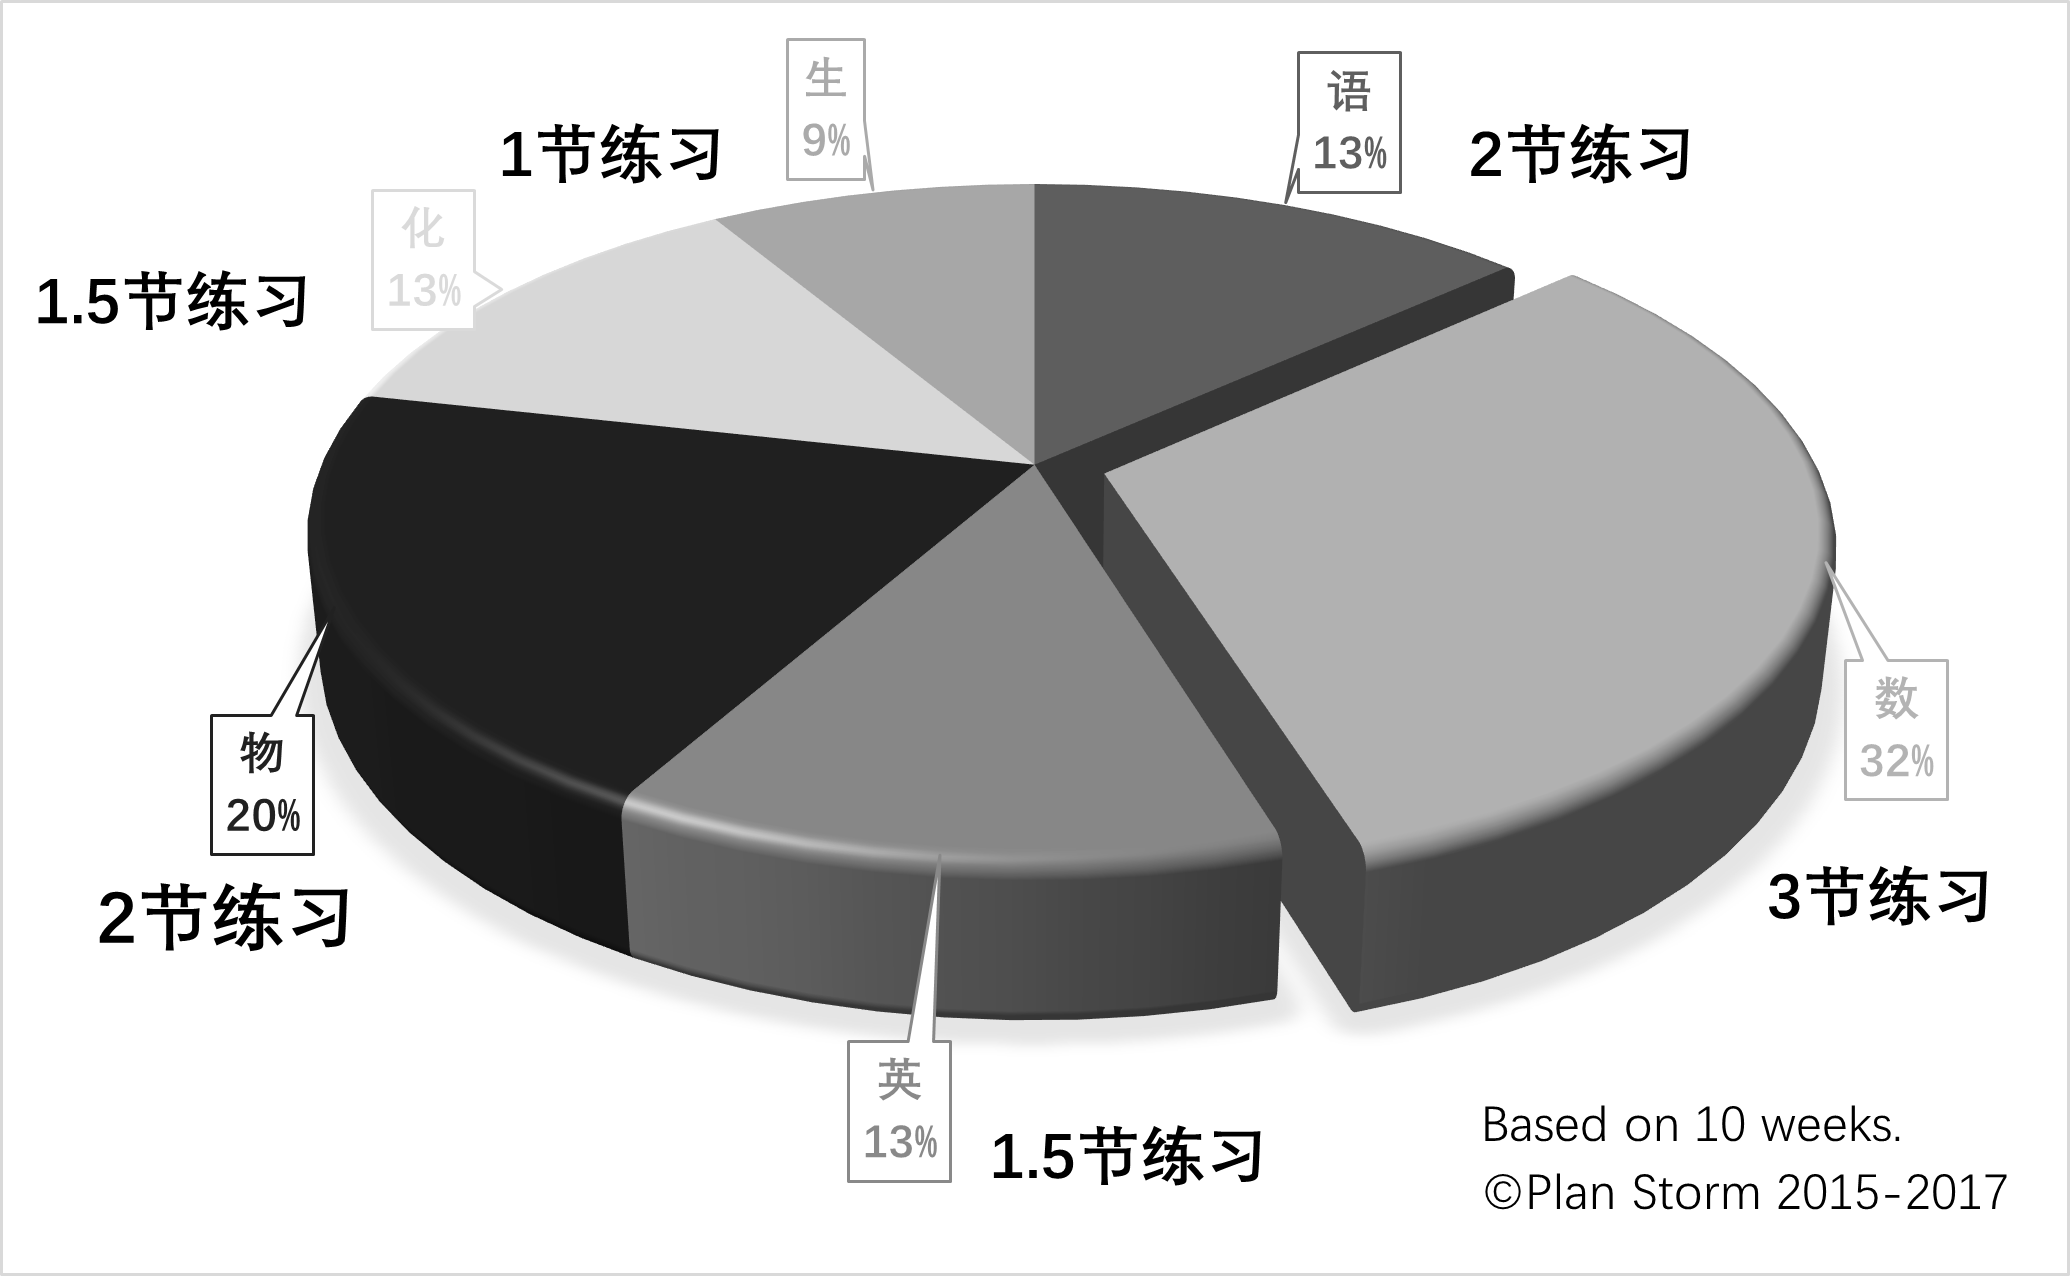
\includegraphics[width=0.8\textwidth]{img/2.png}
    \caption{学科总平均占比}
    \label{ratio}
\end{figure}

\paragraph{3. 作业总量不同的人学科分布有所差异。 } 如图\ref{lv},根据作业总量的不同,将全班化为了3批。右侧表示本批次的平均作业总量。
\begin{itemize}
    \item 纵向看,Lv.3 数学和物理多;Lv.2 语文、英语、生物多;Lv.1 化学多。
    \item 横向看,Lv.3 的作业量比 Lv.1 多50\%。而每周极限平均下来就是23.5小时(这对于任何时候都成立),即每天大约4小时的作业时间(按完成结果算)。
\end{itemize}

\begin{figure}[H]
    \centering
    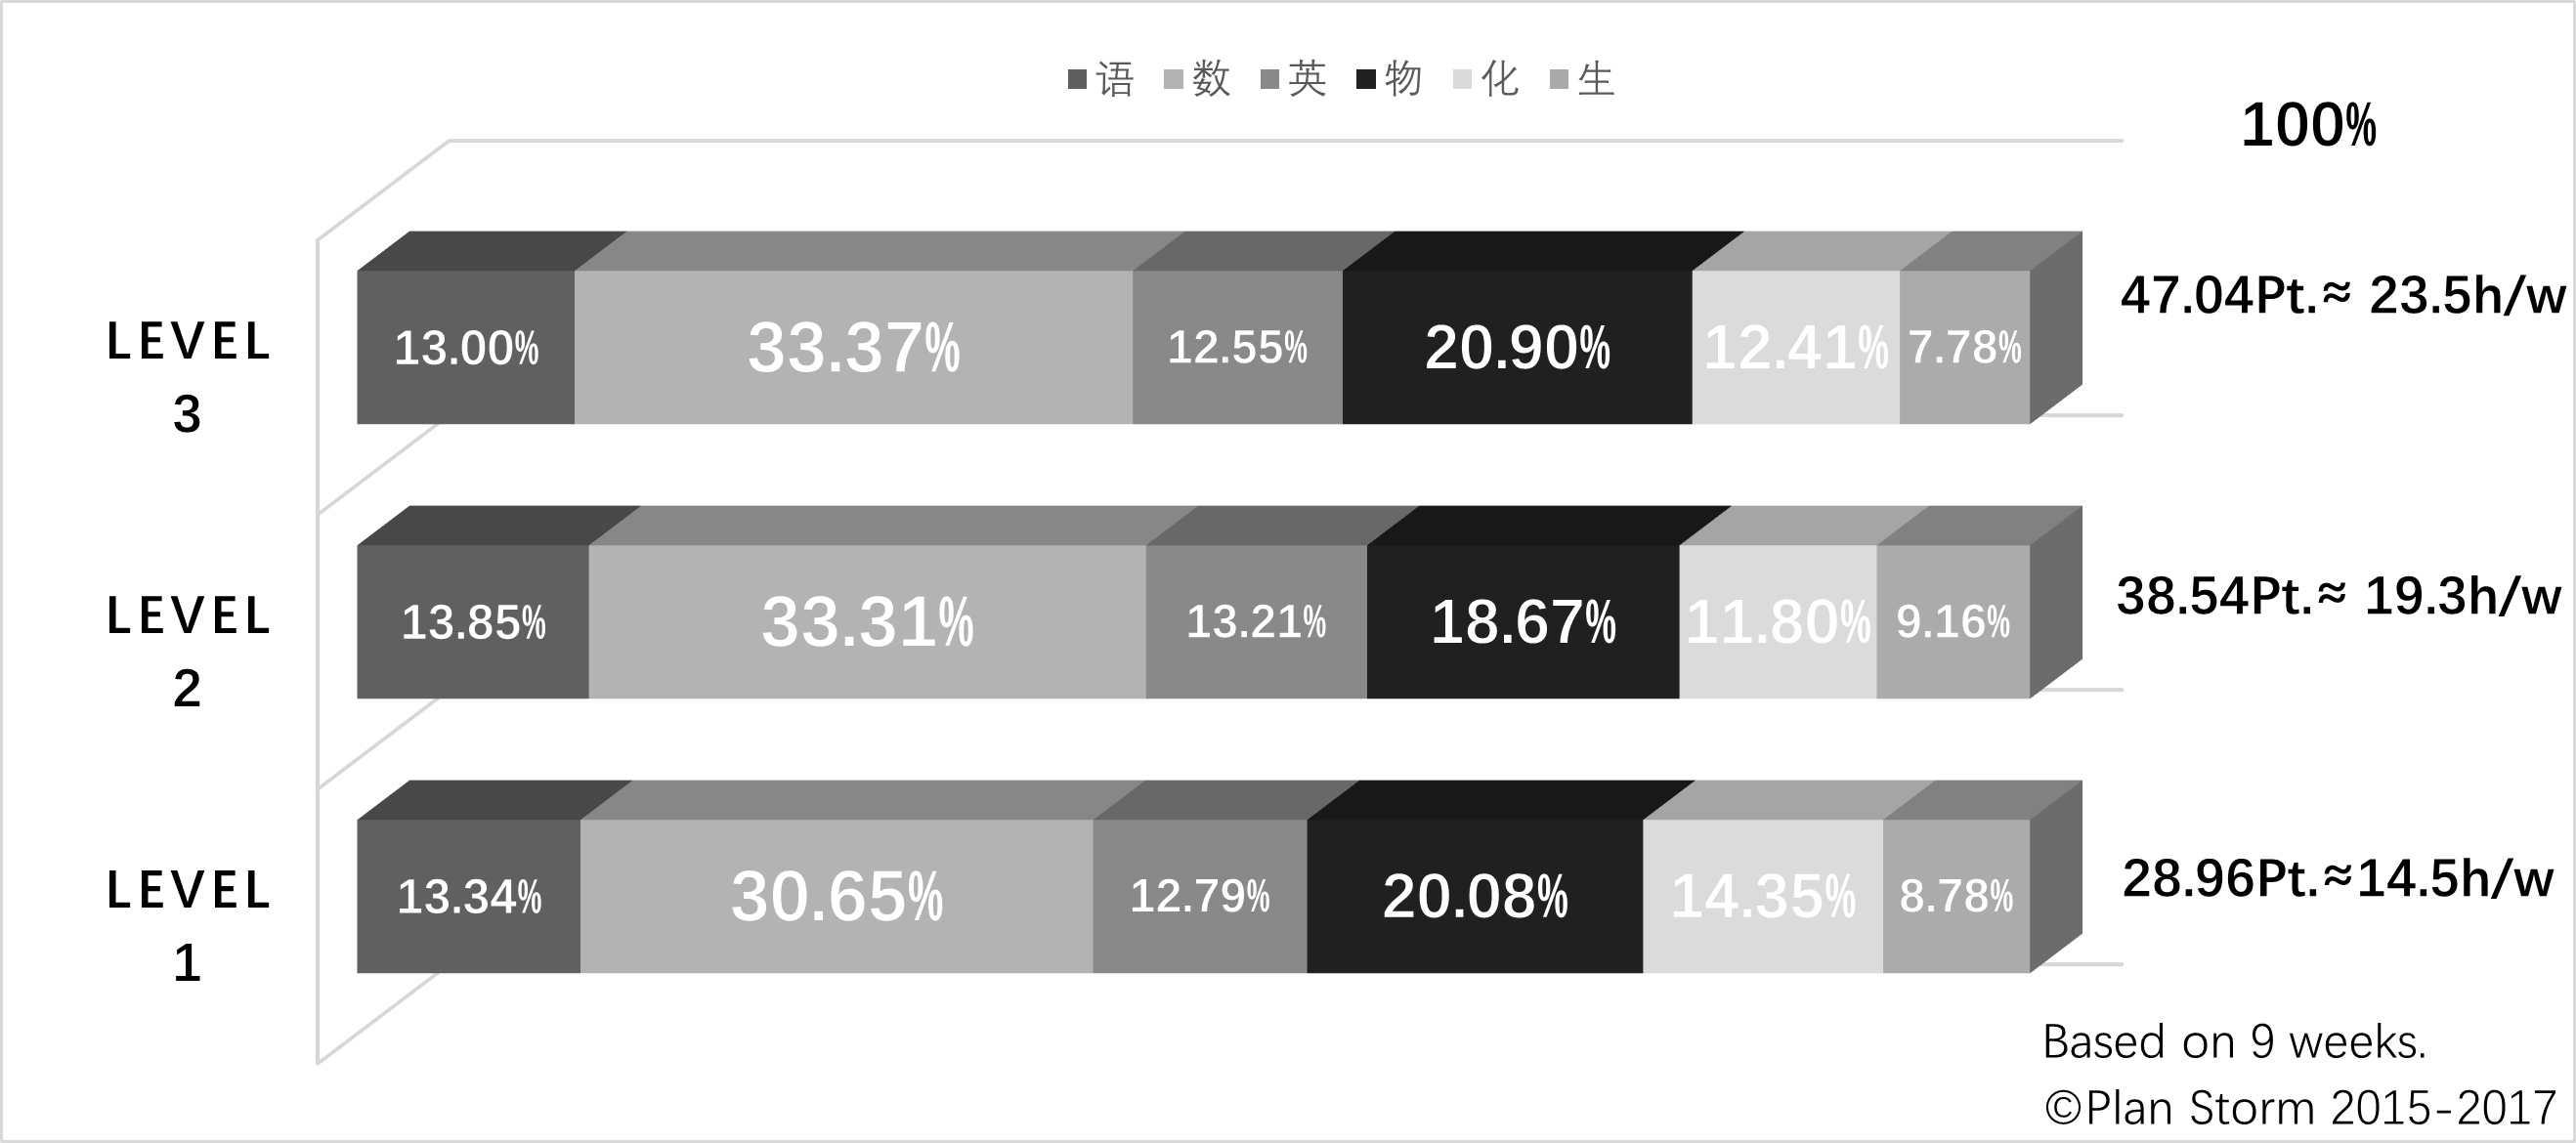
\includegraphics[width=0.8\textwidth]{img/3.png}
    \caption{分批占比}
    \label{lv}
\end{figure}

\begin{table}
    \centering
    \caption{分级9周平均}
    \begin{tabular}{c|rrrrrr}
        Level & 语 & 数 & 英 & 物 & 化 & 生\\
        \hline
         3 & 55.03 & 141.26 & 53.12 & 88.47 & 52.53 & 32.94\\
         2 & 48.03 & 115.53 & 45.82 & 64.76 & 40.91 & 31.76\\
         1 & 34.78 & 79.89 & 33.33 & 52.33 & 37.39 & 22.89\\
    \end{tabular}
\end{table}

\paragraph{4. 每科的每周作业量基本符合正态分布。} 

\begin{figure}[H]
    \centering
    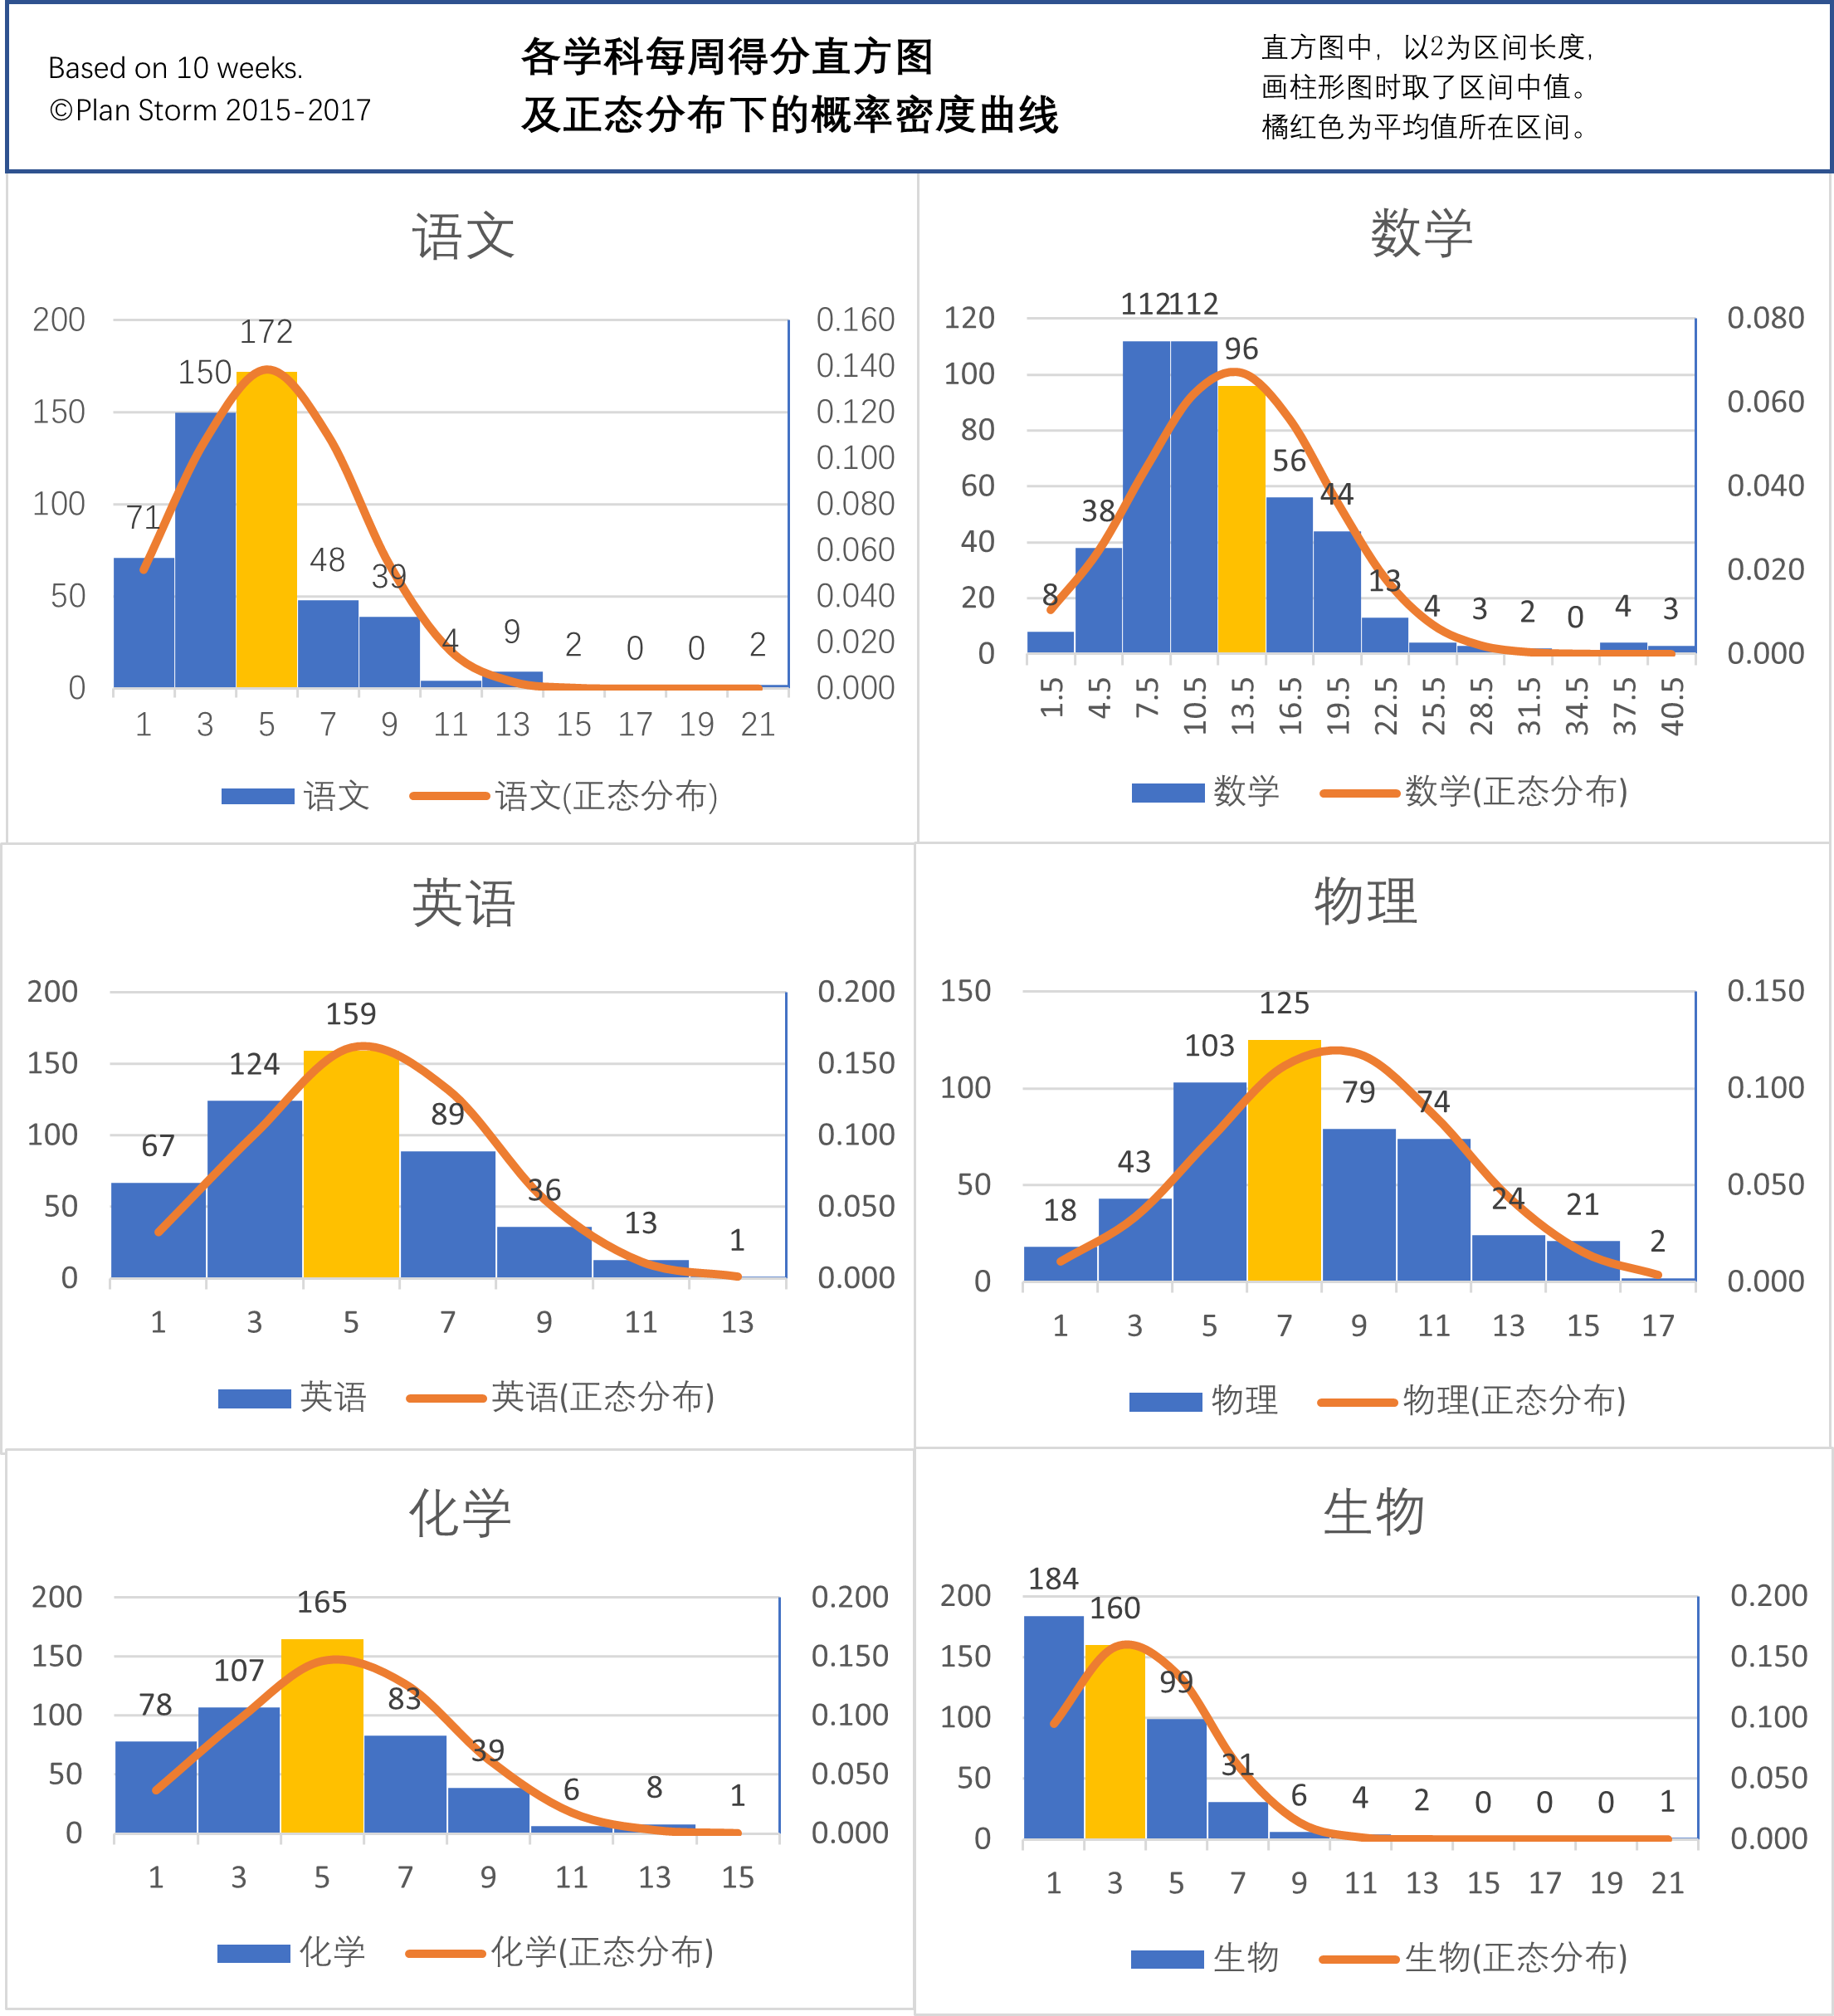
\includegraphics[width=0.9\textwidth]{img/4.png}
    \caption{各学科每周得分(作业量的衡量标准)直方图及正态分布下的概率密度曲线}
    \label{subject}
\end{figure}

由图\ref{subject}可见,其分布于正态分布符合得很好。我们可以将其放在同一个坐标系中。

\begin{figure}[H]
    \centering
    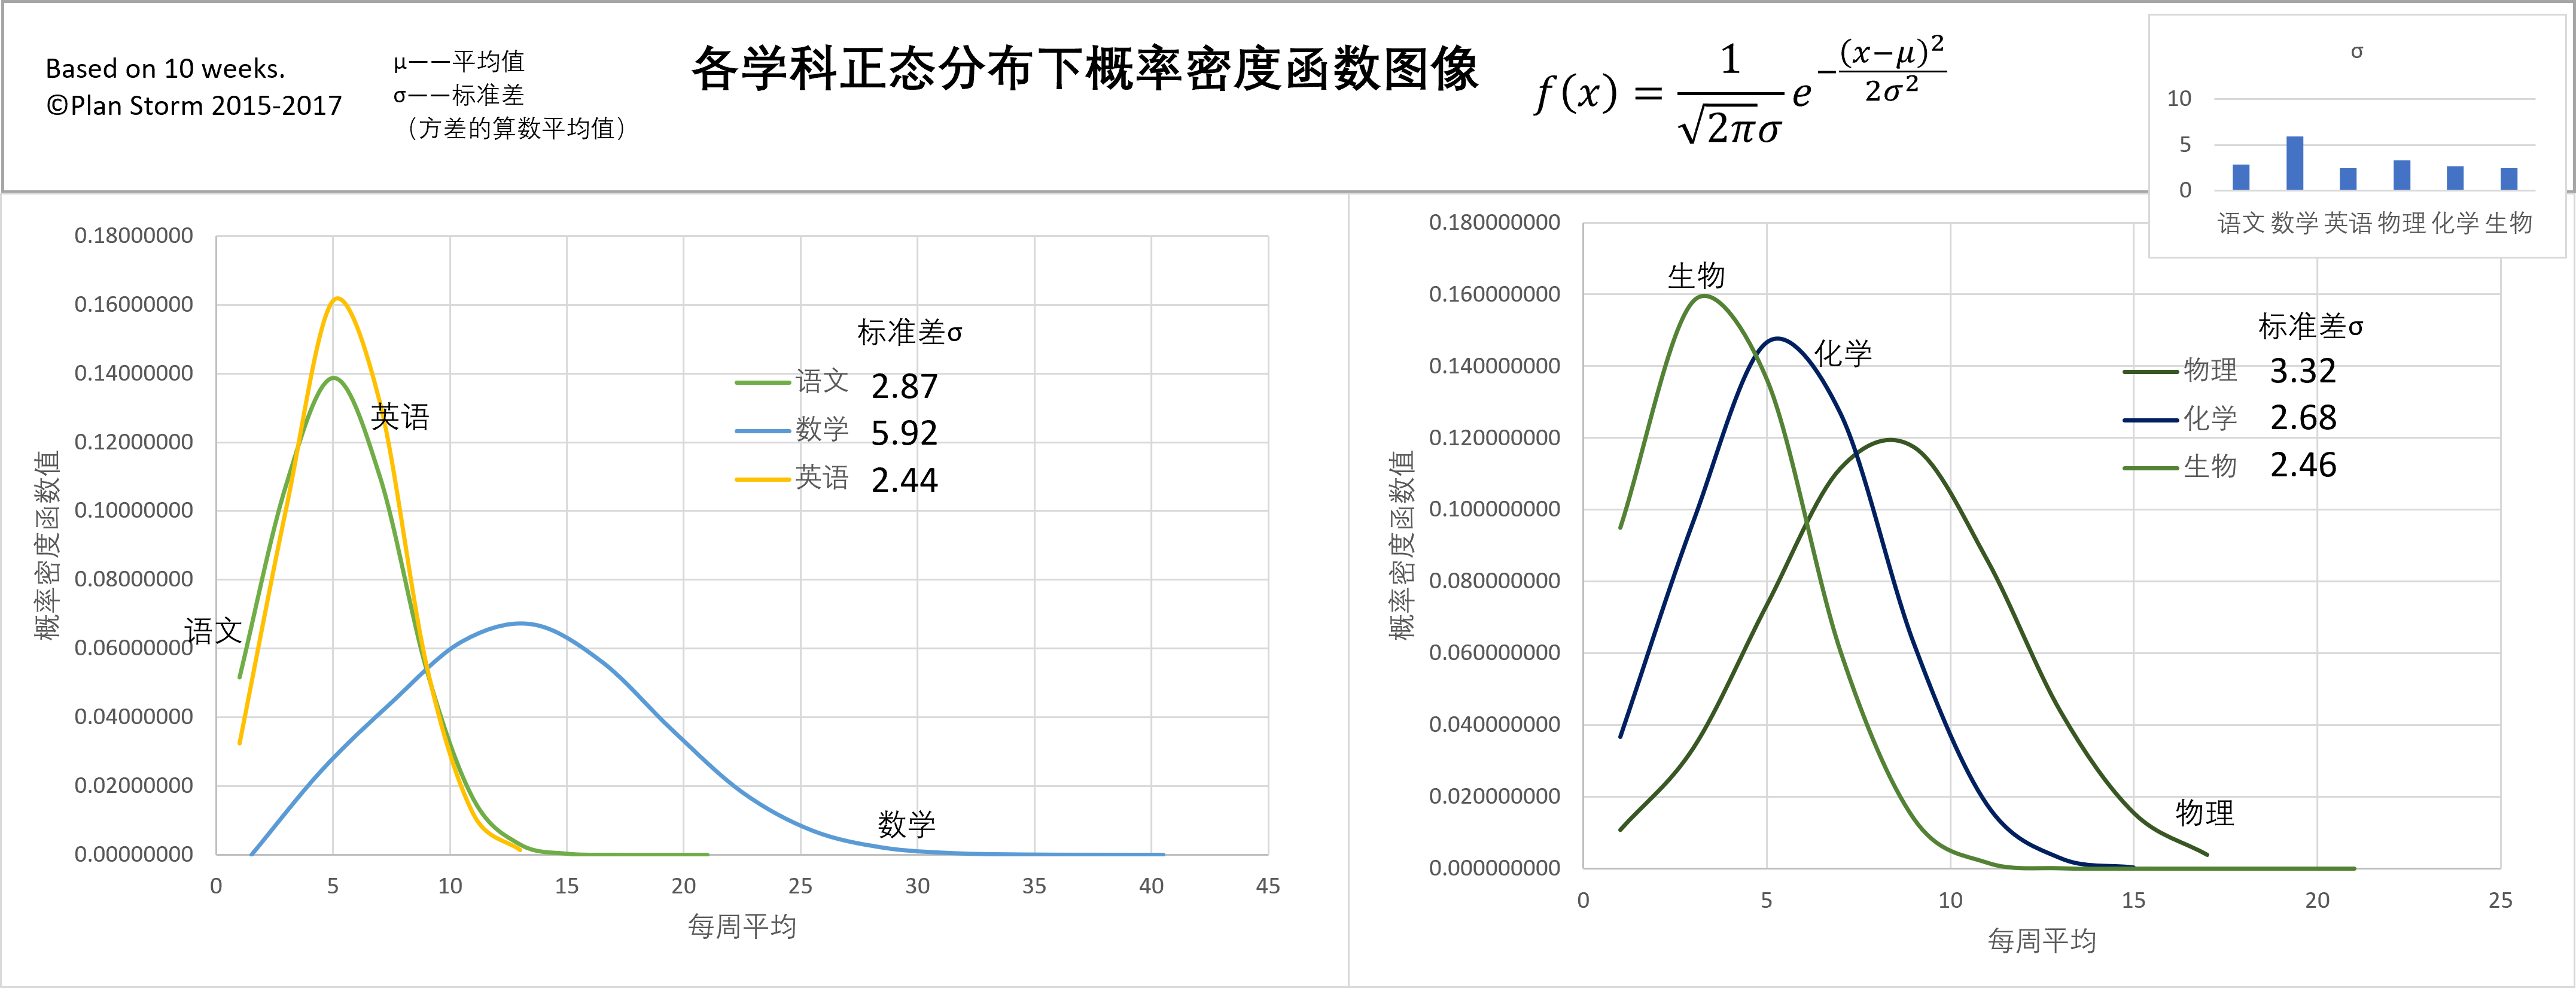
\includegraphics[width=0.9\textwidth]{img/5.png}
    \caption{各学科正态分布下概率密度函数图像}
    \label{var}
\end{figure}

由图\ref{var}可见,数学和物理的完成比较自由(比较“矮胖”),意味着许多同学买了本学科的额外资料并花时间做了;其余学科的完成量区别不大(比较“瘦高”)。

下面附上正态分布下的概率分布列:
\begin{table}[H]
    \centering
    \caption{正态分布下的概率分布列}
    \begin{tabular}{c|rrr}
        $X$ & $[\mu-\sigma,\mu+\sigma]$ & $[\mu-2\sigma,\mu+2\sigma]$ & $[\mu-3\sigma,\mu+3\sigma]$ \\
        \hline
        $P$ & 0.6286 & 0.9544 & 0.9974 \\
    \end{tabular}
\end{table}

\paragraph{5.作业总量是可观的。}
9周下来,作业时间平均为172h,作业量约为344页。1学年(40周)下来,作业量约为1529页(约8本200页厚的书)。

\paragraph{6.结论。} 每周的时间是有限的,所能完成的作业也是有限的。调整方向,将导致另一科低于平均值,而过长时间低于平均,将不利于本学科的发展,推荐波浪形调整形式。
而本文所给出的数据基本是平均的标准。 

\begin{figure}[H]
    \centering
    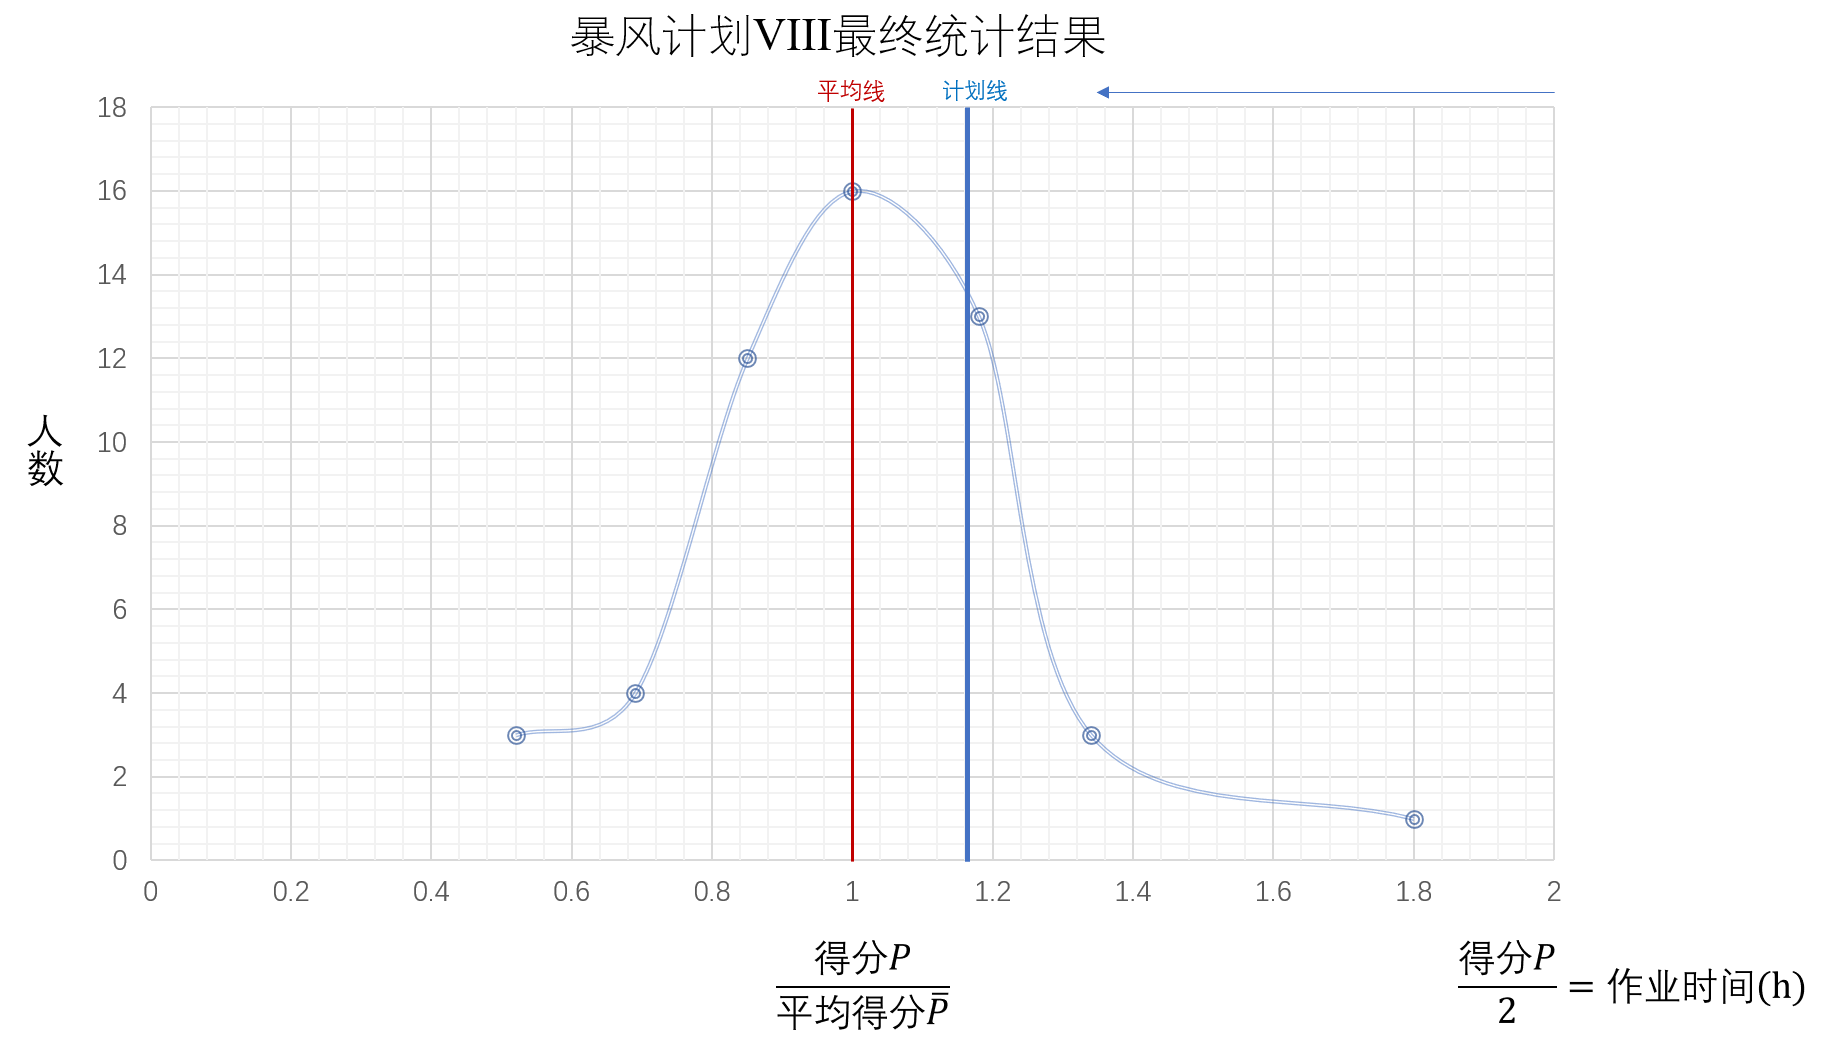
\includegraphics[width=0.75\textwidth]{img/6.png}
    \caption{作业总量分布曲线}
    \label{curve}
\end{figure}

\begin{thebibliography}{}
    \bibitem[1]{}
    百度百科,正态分布,2017
    \bibitem[2]{}
    百度经验,正态分布图像,2017
    \bibitem[3]{}
    LogCreative,暴风计划寒假,2017
    \bibitem[4]{}
    LogCreative,暴风计划技术性报告,2016
    \bibitem[5]{}
    LogCreative,暴风计划(II)颁奖仪式,2015
    \bibitem[6]{}
    LogCreative,暴风计划(IV),2016
    \bibitem[7]{}
    LogCreative,暴风计划(VIII)第一阶段评估,2016
    \bibitem[8]{}
    LogCreative,暴风计划$\rightarrow$新的开始,2017
    \bibitem[9]{}
    LogCreative,日记,2010--2012
    \bibitem[10]{}
    LogCreative,暴风计划阶段性总结,2016
    \bibitem[11]{}
    LogCreative,暴风计划综合期统计,2016
    \bibitem[12]{}
    LogCreative,暴风计划(VIII)统计表,2016
    \bibitem[13]{}
    LogCreative,暴风计划(VIII)统计表1,2017
    \bibitem[14]{}
    LogCreative,暴风计划(VIII)统计表2,2017
    \bibitem[15]{}
    LogCreative,暴风计划(VIII)高三寒假特别计划,2018
\end{thebibliography}
    

\end{CJK}
\end{document}